\documentclass[
    corpo=12pt,
    oneside,
    evenboxes,
    tipotesi=triennale,
    stile=classica,
    oldstyle,
    autoretitolo,
    greek,
]{toptesi}
\usepackage[utf8]{inputenc}
\usepackage[T1]{fontenc}
\usepackage{lmodern}
\usepackage{hyperref}
\usepackage{setspace}
\usepackage{verbatim}
\usepackage{pgfplots}
\usepackage{graphicx}
\usepackage{subfig}
\onehalfspacing

\hypersetup{
    pdfpagemode={UseOutlines},
    bookmarksopen,
    pdfstartview={FitH},
    colorlinks,
    linkcolor={blue},
    citecolor={blue},
    urlcolor={blue}
  }
\usepackage{lipsum}

\newtheorem{osservazione}{Osservazione}

\begin{document}\errorcontextlines=9

\begin{ThesisTitlePage}
    \ateneo{Universit\`a degli Studi di Torino}
    \StrutturaDi{Dipartimento di Management}
    \struttura[]{}
    \NomeElaborato{Tesi di laurea triennale}
    \titolo{Fair Play Fiananziario e Superlega}
    \sottotitolo{Lo stato di salute del Calcio pre e post COVID-19}     
    \corsodistudi{Management dell'Informazione e della Comunicazione Aziendale}
    \candidato{Riccardo \textsc{Borgo}}
    \relatore{prof.ssa ~Simona \textsc{Alfiero}}
    \sedutadilaurea{\textsc{Anno~accademico} 2021-2022}
    \logosede{img/Unito-logo, img/logo_saa.jpeg}
\end{ThesisTitlePage}

\figurespagetrue
\indici

\mainmatter
\begin{interlinea}{1.5}
    
\chapter{Introduzione generale}
Durante lo sviluppo di questa trattazione si andrà ad analizzare l'attuale "stato di salute"
del calcio europeo, di come il \emph{Financial Fair Play} abbia provato da una parte ad aiutare le società a rimanere in regola con i conti e 
dall'altra a dettare delle regole atte ad evitare comportamenti illegali da parte sopratutto dei presidenti.\\
Infine si tratterà il caso della \emph{Superlega}, per cercare di capire se questa nuova idea sia effettivamente coerente con l'epoca in cui stiamo vivendo.\\
Sopratutto a partire dall'inizio della pandemia da COVID-19 nei primi mesi del 2020 il mondo del calcio si è visto ridurre sensibilmente i ricavi, non riuscendo 
ancora oggi ad operare al 100\%. Grazie, forse, a questa situazione di difficoltà è stato evidenziato come la situazione odierna non fosse più sostenibile: 
club con milioni di euro di debiti, richieste di ingaggio "faraoniche" da parte dei calciatori, con il risultato che molte societ\`a non sono state pi\`u in grado di far fronte 
a tutto questo e costrette a dichiarare falimento.\\
Il primo capitolo mira ad analizzare la situazione economica, finanziaria e patrimoniale, antecedente all'anno 2020 di alcune delle più 
importanti e storiche societ\`a di tutto il panorama europeo: Juventus per quanto riguarda l'Italia, Paris Saint Germain per quanto riguarda la 
Francia, Bayern Monaco per la Germania, Manchester City per l'Inghiterra e il Barcellona per la Spagna. I punti principali dell'analisi riguarderanno: 
Analisi dei ricavi, Analisi della liquidit\'a, Analisi della solidit\'a, Analisi della redditivit\'a e Trend azionario (se presente) in modo da 
poter fare una verifica a 360° di tutti i vari settori economici. La scelta \'e virata su queste societ\'a perch\'e per un motivo o per un altro sono state 
al centro di problematiche o scandali legate alla cattiva gestione del patrimonio oppure "accusate" di non essere state prese particolarmente prese di mira dalle misure e le leggi 
emanate nell'ultimo decennio dalla UEFA \footnote{ Union of European Football Associations}, come per esempio il \emph{Financial Fair Play}.\\
Il secondo capitolo si occuper\'a invece della presentazione e dell'analisi in modo dettagliato del \emph{Financial Fair Play} o 
\emph{FFP}, dalla sua nascita, alle varie parti presenti all'interno del documento e mostrando infine come, non sempre, tutte le societ\'a siano state trattate allo stesso modo.\\
Il terzo capitolo invece analizza invece l'impatto mediatico, non prima di aver presentato tutti i dati tecnici, di una delle ultime novità 
del mondo del calcio: la \emph{Superlega}: il nuovo modello che punta a rivoluzionare il mondo del calcio, per cercare di uscire da questa spirale di debiti
e fallimenti per cercare quindi di creare un nuovo inizio. Verr\'a mostrato in seguito se il progetto ha effettivamente preso piede all'interno del mondo del calcio 
e se è riuscito a smuovere qualcosa, portando agli occhi di tutti l'insostenibilità del modello attuale.\\
In chiusura si cercherà di determinare se i rimedi proposti dalle autorità del mondo del calcio siano stati sufficienti ad eliminare tutte le criticità presenti e 
sopratutto evidenziare l'impatto economico di questi rimedi.\\
Riuscir\'a la Superlega ad acquistare credibilità e ad affermarsi come nuovo modello, capace di risollevare il calcio?

\part{Parte Prima}
\chapter{Situazione economica Europea pre-pandemia da COVID19}
\section{Analisi generale delle diverse realt\'a Europee}
Prima di andare ad analizzare nello specifico i vari club europei \'e necessario iniziare con una prima 
parte atta a presentare la situazione generale all'interno di ogni Paese. Verrà mostrato come non in tutti 
si riesca ad arrivare ad un risultati positivo, andando quindi a rendere in qualche modo 
"unico" ogni campionato e la sua relativa Federazione. Le Federazioni (uniche per ogni Stato) hanno tendenzialmente il compito
comune di organizzare i campionati nazionali e designare gli arbitri per i vari incontri. Oltre a questo compito pi\'u di tipo
organizzativo le varie Federazioni hanno il dovere di garantire un accesso libero ed universale al gioco del calcio, senza distinzioni
di genere ed etnia. Questi due compiti \'e possibile estrapolarli dagli 11 punti contenenti i valori che la UEFA 
\footnote{Wikipedia: Union of European Football Associations, raggruppa tutte le Federazioni dei vari stati Europei e non} vuole
trasmettere tramite la sua attivit\'a \footnote{Wikpedia: https://it.wikipedia.org/wiki/Union\_of\_European\_Football\_Associations, I Valori UEFA}.\\
L'analisi verter\'a principalmente su due settori: \textbf{Risultato Economico 2019} e \textbf{analisi degli stipendi}; questi due elementi
permettono di generare un'opinione abbastanza completa perch\'e da un lato si evidenzier\'a come si \'e giunti a quel risultato (entrate e spese)
e dall'altra si analizzer\'a uno dei temi pi\'u discussi di sempre riguardo il mondo del calcio, andando a capire se gli stipendi dei calciatori
siano collegati o meno ai risultati ottenuti.\newline
Il primo paese preso in esame \'e l'\textbf{Italia}, la quale presenta una situazione decisamente non ottimale. La gestione del sistema calcio 
\'e affidata alla FIGC\footnote{Federazione Italiana Giuoco Calcio} che si è rivelata nel corso degli anni addirittura legata ad affari illeciti:
il pi\'u eclatante sicuramente il caso \emph{Calciopoli} datato 2006 che ancora oggi non ha prodotto un vero colpevole ma ha comunque portato
alla dimissione dell'allora Presidente e Vicepresidente Franco Carraro e Innocenzo Mazzini\footnote{Wikipedia: https://it.wikipedia.org/wiki/Calciopoli}.
Tornando ad un'analisi prettamente economica, la sezione dei \textbf{Ricavi} a partire dalla stagione 2013/2014 ha sempre registrato un valore 
in crecita, passando da 2625mln€ nel 2013/2014 a 3854mln€ nel 2018/2019 (incremento del 46\%)\footnote{FIGC: https://www.figc.it/it/federazione/federazione-trasparente/reportcalcio/}. 
Anche se i dati riportano un valore complessivamente in linea con la maggior parte degli altri Paesi, il fatto che non rassicura \'e che non
ci sia mai stata la capacit\'a di avere un valore di ricavi che superasse quello dei costi. La voce che abbatte maggiormente il valore 
della produzione (primo addendo della somma algebrica che genera il Risultato Netto) sono gli ammortamenti che, nel caso del calcio, 
si riferiscono al costo del cartellino dei calciatori (costo storico) e il loro relativo contratto (vita utile). L'aumento di questa voce
non \'e quindi necessariamente un aspetto negativo perch\'e spiega come le societ\'a vogliano investire molto per il miglioramento delle
rose; il problema sorge per\'o se non si ottengono risultati in campo internazionale. Quest'ultimi generano importanti 
ricavi per le societ\'a e spesso sono proprio loro che consentono alle societ\'a di crescere economicamente. lL'ultimo successo in campo 
internazionele da parte di una squadra italiana risale al 2010 con la vittoria della Champions League da parte dell'Inter e, a parte
le due finali raggiunte dalla Juventus non ci sono stati altri traguardi degni di nota da parte dei team italiani in Europa.\newline
Passando invece all'argomento \textbf{stipendi} la FIGC non fornisce un resoconto dettagliato riguardo gli stipendi dei tesserati durante l'anno; 
l'unico spunto di analisi pu\'o essere estrapolato dall'approfondimento sulle voci di costo anche se quest'ultima non consente di fornire 
un'opinione a 360° dell'argomento, poich\'e, se si osserva solamente il grafico ripreso dalla figura \ref{figA} si potrebbe constatare come
non ci siano particolari debolezze dato che il peso degli stipendi rimane costante. Il problema sorge osservando la figura accanto \ref{figB}
\footnote{Ultimo Uomo: https://www.ultimouomo.com/guida-ai-monte-ingaggi-della-serie-a-2018-19/} che mostra come due societ\'a abbiano
abbattuto il tetto dei 100mln€ di ingaggio per i calciatori e di come altre 3 societ\'a ci siano andate molto vicino. complessivamente
troviamo un generale aumento degli stipendi dovuto principalmente ai maggiori
introiti da diritti tv grazie all'arrivo del calciatore Cristiano Ronaldo alla Juventus.\newline
\begin{figure}
    \centering
    \subfloat[][Composizione dei costi all'interno del sistema calcio italiano]
    {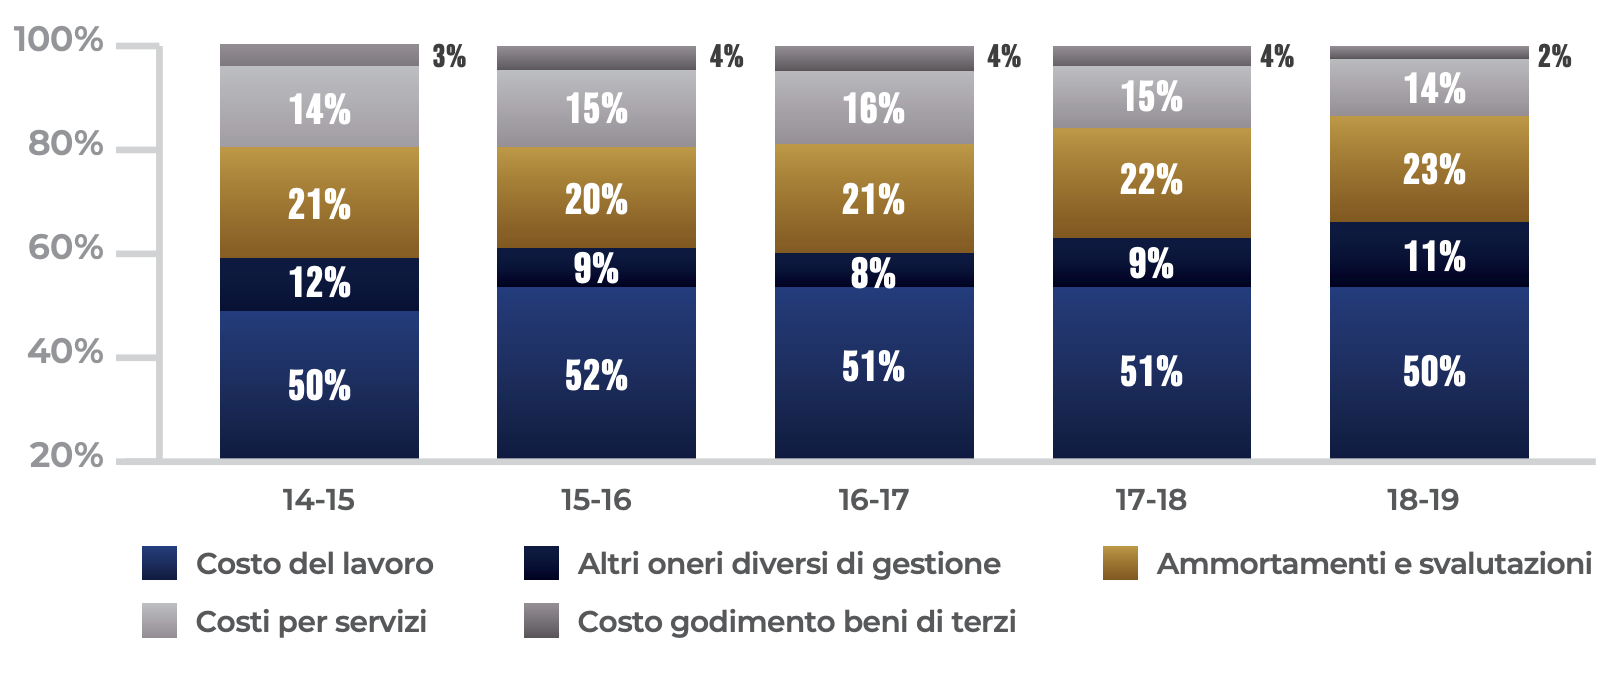
\includegraphics[width=.55\textwidth]{img/wage_serieA.png} \label{figA}} \quad
    \subfloat[][Confronto stipendi Serie A 17/18 e 18/19]
    {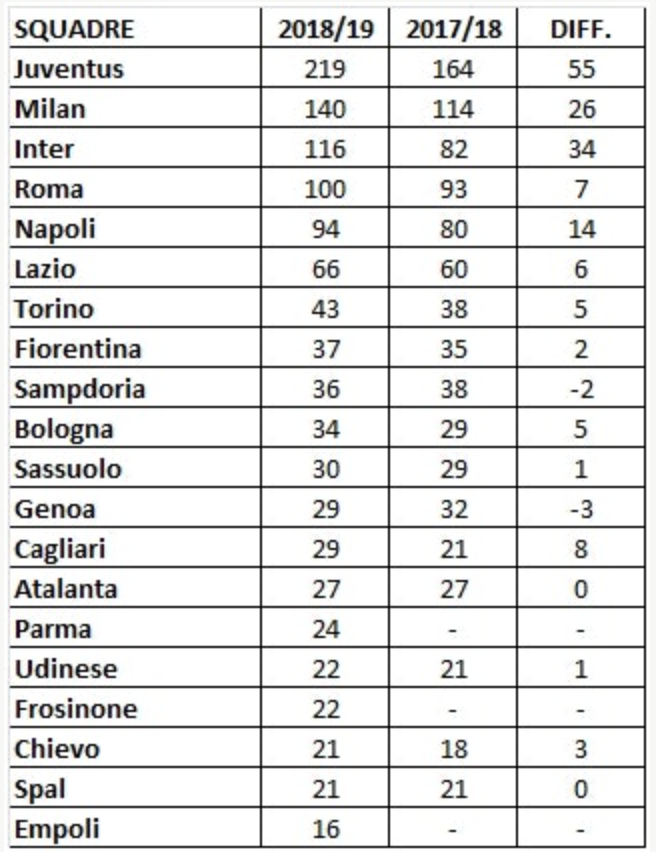
\includegraphics[width=.25\textwidth]{img/diff_wage_serieA.png} \label{figB}}
    \caption{Situazione \emph{Costo del Lavoro} all'interno del calcio italiano}
    \label{wage_serieA}  
\end{figure}
Il problema \'e che questo momento di respiro sar\'a solo qualcosa di temporaneo, che scomparir\'a quando Cristiano Ronaldo e la 
sua immagine non saranno pi\'u legati alla Serie A.\newpage
Per quanto riguarda invece la \textbf{Francia}, l'organizzazione che si occupa del monitoraggio e la supervisione dei conti 
delle società calcistiche è la DNCG\footnote{Direction Nationale du Contrôle de Gestion}. Essa 
pubblica ogni stagione un report riassuntivo per quanto riguarda la Ligue 1 e la Ligue 2 (i primi due campionati francesi) ed una
relazione relativa ad ogni singolo club dei due campionati. Tutti i dati di seguito riportati sono stati reperiti dai singoli
report annuali pubblicati\footnote{https://www.lfp.fr/dncg/rapports} \newline 
La perdita registrata nella stagione 18/19 che ammontava a 126mln€ \'e la seconda in termini di importanza a partire dalla stagione 2013/2014.
Il motivo principale che spiega questa discesa cos\'i decisa, \'e da attribuirsi ad un aumento delle entrate (\emph{Income})
da 304 mln€ nel 17/18 a 316 mln€ nel 18/19, che per\'o non riesce a contrastare l'aumento pi\'u elevato
delle spese (\emph{Expenses}) sopratutto nella sezione dedicata alle spese proprie dei club: stipendi di giocatori e commissioni degli agenti 
in cui troviamo un aumento rispetto all'anno precedente di 9 mln€.\newline
Il secondo indicatore che viene preso in considerazione \'e chiamato \textbf{Payroll}, termine indicante la somma dei vari stipendi
dei dipendenti di un club. Nonostante un Payroll, almeno per quanto riguarda le squadre qualificate per la UCL \footnote{Uefa Champions League}, in linea con gli
altri campionati (147 mln€ nella Premier League inglese \footnote{Calcolo personale utilizzando i dati da https://www.spotrac.com/epl/payroll/})
i risultati ottenuti nelle competizioni internazionali non sono state all'altezza: nella stagione 2018/2019 sono presenti 3 squadre 
all'interno della fase a gironi della massima competizione europea: Monaco, Paris Saint Germain e Olympique Lione. La prima si 
posizione ultima nel gruppo A, la seconda (da cui gli esperti e i sostenitori si aspettano grandi risultati, visti i milioni di euro 
spesi ogni anno) viene eliminata agli ottavi di finale e infine la terza viene anch'essa eliminata agli ottavi di finale. Questo scenario
si ripete mediamente ogni anno, inoltre, se si vuole trovare una squadra francese vincitrice dobbiamo tornare indietro alla stagione 1992/1993
con l'Olympique Marsiglia. La figura \ref{stipendi_ligue1} permette di capire, oltre alla disparit\'a di risorse in possesso dei club in Francia, 
anche il livello di spesa dei club per gli stipendi, che come \'e stato detto in precedenza non viaggia di pari passo ai traguardi interazionali.\newline
\begin{figure}
    \centering
    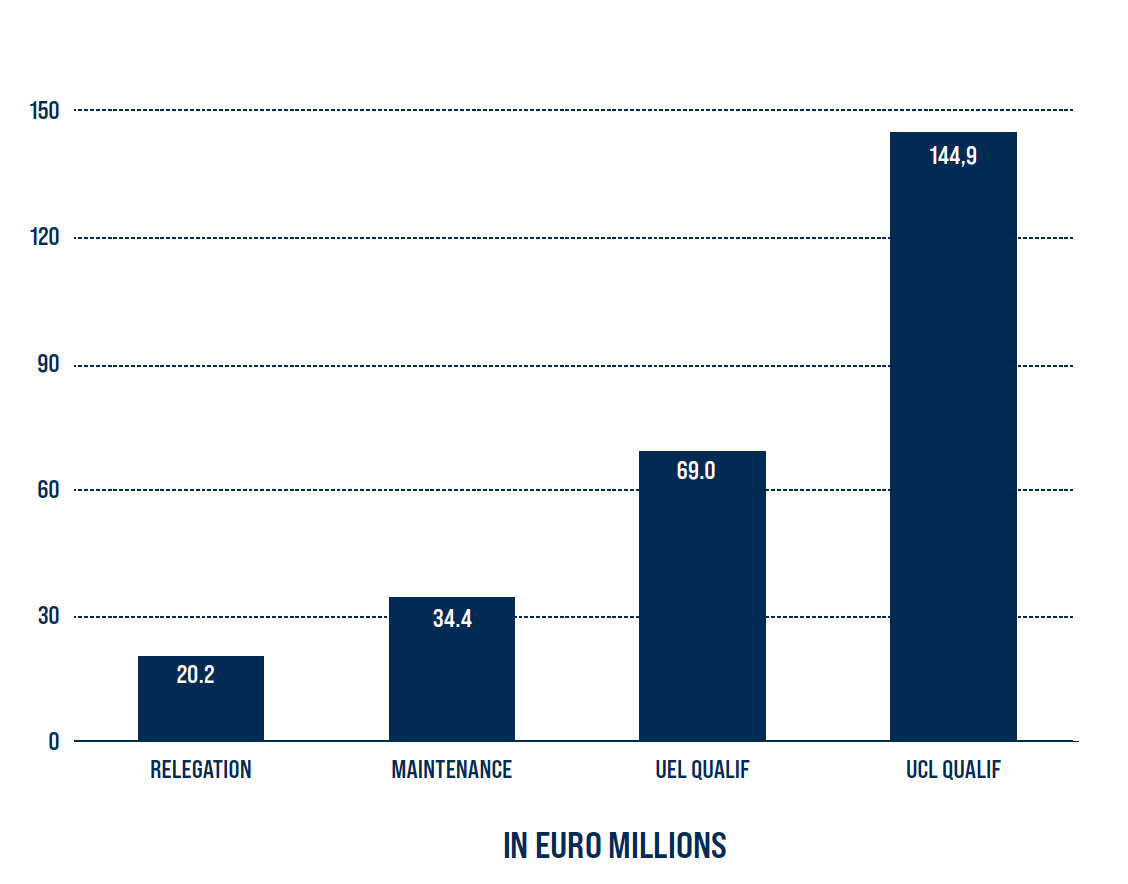
\includegraphics[scale=0.5]{img/stipendi_ligue1.png}
    \caption{Stipendi Ligue 1 a seconda del piazzamento in classifica}
    \label{stipendi_ligue1}
\end{figure}
Riprendendo l'ultimo indicatore analizzato e collegandolo al primo \'e possibile constatare, come per l'Italia, che i grandi investimenti spesso non portano 
al successo assicurato e quindi ad un ritorno concreto. Queste grosse somme che escono dalle casse dei club che per\'o
non vedono un ritorno portano un danno a tutto il campionato, perch\'e da un lato viene aumentato il gap tecnico tra le diverse squadre dello
stesso campionato mentre dall'altro, in campo internazionale, non si ottengono risultati non ricevendo quindi premi da sponsor e organizzatori.
Tutto questo circolarit\'a non fa' altro che danneggiare il sistema calcio francese perch\'e si fa perdere valore e quindi appeal, sia 
visivo che economico, al campionato locale e si "danneggia" l'immagine europea dei club francesi, considerati incapaci, nonostante le somme spese,
di ottenere risultati.\newline
Il terzo Paese e di conseguenza ambiente calcistico che verr\'a analizzato \'e la \textbf{Germania}, dove troviamo la \emph{Bundesliga} e la \emph{2.Bundesliga} 
cio\'e i primi due campionati per ordine di importanza che vengono raggruppati sotto la DFL\footnote{Wikipedia: Deutsche Fußball Liga}, la
federazione calcistica tedesca.\newline
Questo campionato, come pochi in Europa, possiede davvero poche criticit\'a. Iniziando con l'analisi del risultato, 
esso \'e uno degli elementi che pi\'u di tutti gli altri viene pubblicizzato 
da parte della Lega stessa all'interno del Report Annuale: 4.82 mld€ di ricavo generato dai primi due campionati nazionali in un 
solo anno, spiegato come un grande traguardo raggiunto e che rimane inoltre un primato da 15 anni consecutivi
\footnote{https://www.dfl.de/en/2018-dfl-report/}.\newline
I \textbf{Ricavi} della Bundesliga sono cresciute da 2.59 mld€ nel 2016/2017 a, come detto in precedenza, 4.82 mld€ nel 2018/2019, 
registrando quindi un incremento dell'85.32\% nei 5 anni e dell'8.5\% rispetto
all'anno precedente. Entrando nel dettaglio, sono aumentati i ricavi dai media grazie ai maggiori contratti nazionali siglati dalla stagione precedente tuttavia sono diminuiti, anche se di poco,
i ricavi da pubblicit\'a e incontri, imputabile in modo prevalente ad un cambio della composizione del campionato stesso.
Questi ottimi risultati vengono anche supportati dal dato dei club con risultato positivo a fine esercizio: 28 su 36 (considerando 
Bundesliga e 2.Bundesliga) nel 2018/2019, mostrando come in questo Paese tutte le societ\'a, partendo dalle pi\'u virtuosi 
come il Bayern Monaco, fino ad arrivare a realt\'a pi\'u modeste come per esempio l'Erzgebirge Aue militante nel secondo campionato.\\
Passando alla seconda parte dell'analisi, \textbf{gli stipendi}, essi non seguono lo stesso ragionamento fatto poco prima: la figura 
\ref{comparazione_stipendi_germania} mostra come, nonstante il valore complessivo degli stipendi dei calciatori e staff sia cresciuto in entrambi
i campionati, il totale della Bundesliga sia circa maggiore di 7 volte rispetto al campionato minore, andando quindi a dimostrare
un grande scalino di differenza tra le due leghe.
\begin{figure}
    \centering
    \subfloat[][Bundesliga]
    {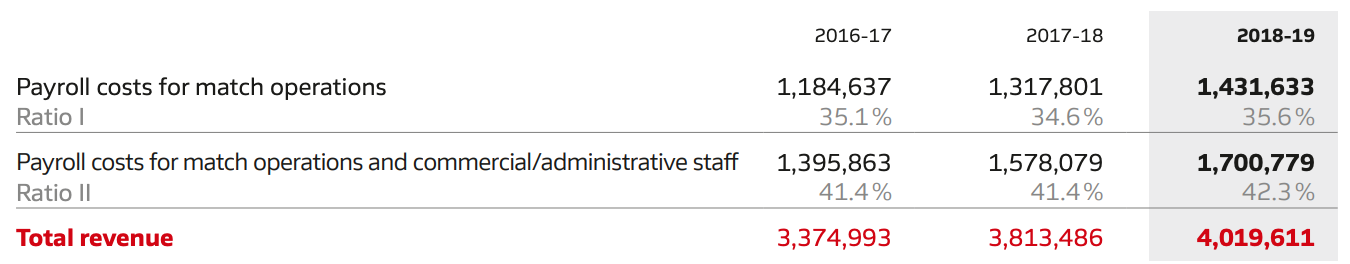
\includegraphics[width=.65\textwidth]{img/wage_germanyA.png} \label{wage_germanyA}} \quad
    \subfloat[][2.Bundesliga]
    {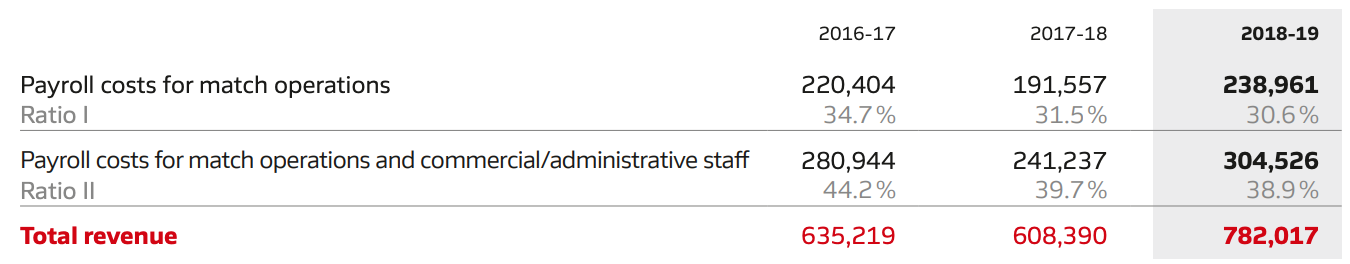
\includegraphics[width=.65\textwidth]{img/wage_germanyB.png} \label{wage_germanyB}}
    \caption{Comparazione stipendi con storico}
    \label{comparazione_stipendi_germania}  
\end{figure}
In Germania \'e radicata sicuramente una cultura legata alla precisione e al rispetto sia delle leggi che delle persone, questo si riflette 
ovviamente in tutti gli ambiti compreso quello del calcio. Come \'e possibile notare, in questo caso, i club prestano molta attenzione a non 
terminare l'anno economico con elevati debiti oppure con risultati ad un passo dal fallimento, nonostante queste attenzioni, al contrario
di come si potrebbe pensare, arrivano anche risultati dal campo poich\'e negli ultimi anni le squadre tedesche sono sempre riuscite a ritagliarsi 
il proprio spazio nelle competizioni europee, spazio riempito con la vittoria della Champions League da parte del Bayern Monaco nel 2020. 
Rimane sempre per\'o il problema dell'inequit\'a degli stipendi. \'E possibile tuttavia anticipare gi\'a da ora, come in nessuno stato, non si possa
trovare similitudini in termini economici tra i primi due campionati per ordine di importanza.\newline
Come penultimo campionato oggetto dell'analisi troviamo la \textbf{Spagna}, formato dalla prima divisione \emph{La Liga Santander} e la seconda
\emph{La Liga Smartbank} \footnote{Tutti i dati provengono da: https://www.laliga.com/en-GB/transparency/economic-management/economic-report}.
Il Reddito Complessivo dei due campionati registra una crescita 
dalla stagione 2013/2014. Si parte con un valore combinato di 2688.5 mln€ e si arriva alla stagione 18/19 con un totale di 4871.4 mln€, 
un incremento dell'81,19\%. 
Suddividendo in modo settoriale il Total Income \'e possibile capire come in tutti i vari settori che compongono il Total Income 
si sia verificato un aumento rispetto agli anni precedenti, andando a mostrare quindi come il campionato spagnolo abbia vissuto una forte crescita negli ultimi 6 anni.
I settori sono:
\begin{enumerate}
    \item \textbf{Trasmissioni}: 1665.1 mln€ (+6.2\% rispetto all'anno precedente e +13.6\% in 5 anni). Questa crescita \'e dovuta sopratutto ad una distribuzione 
    centralizzata dei diritti grazie al RDL 5/2015 \footnote{Wikipedia: Real Decreto Ley è un atto avente forza di legge emanato dal Re}.
    \item \textbf{Attivit\'a commerciali}: 983.8 mln€ (+5.5\% rispetto all'anno precedente e +16.7\% in 5 anni). Comprende sponsorizzazioni,
    pubblicit\'a e merchandising.
    \item \textbf{Partite}: 948.6 mln€ (+24.4\% rispetto all'anno precedente e +9.3\% in 5 anni). Comprende le competizioni, biglietti 
    e altre entrate distribuite dalla UEFA.
\end{enumerate}
Il risultato finale del Reddito \'e stato, inoltre, favorito in modo importante dalla crescita di altri 2 fattori che caratterizzano l'attivit\'a tipica del
campionato:
\begin{enumerate}
    \item \textbf{Trasferimenti}: 1,006.2 mln€ (+7.2\% rispetto all'anno precedente e +18.1\% in 5 anni).
    \item \textbf{Altre Entrate}: : 267.7 mln€ (+15.7\% rispetto all'anno precedente e -2.8\% in 5 anni). Unico valore che vede una diminuzione
    nel medio periodo ma dovuta al fatto che questa voce, comprendendo accordi di natura finanziaria, assume valori molto diversi nel corso degli anni.
\end{enumerate}
Spostandosi al secondo tema, anche in questo caso come per l'Italia, non viene elaborata un'analisi dettagliata degli stipendi. Nel documento
viene indicato solamente il costo degli stipendi nel corso degli anni e il suo rapporto in percentuale con il Reddito Complessivo e il Fatturato Netto
(figura \ref{wage_spain}).
\begin{figure}
    \centering
    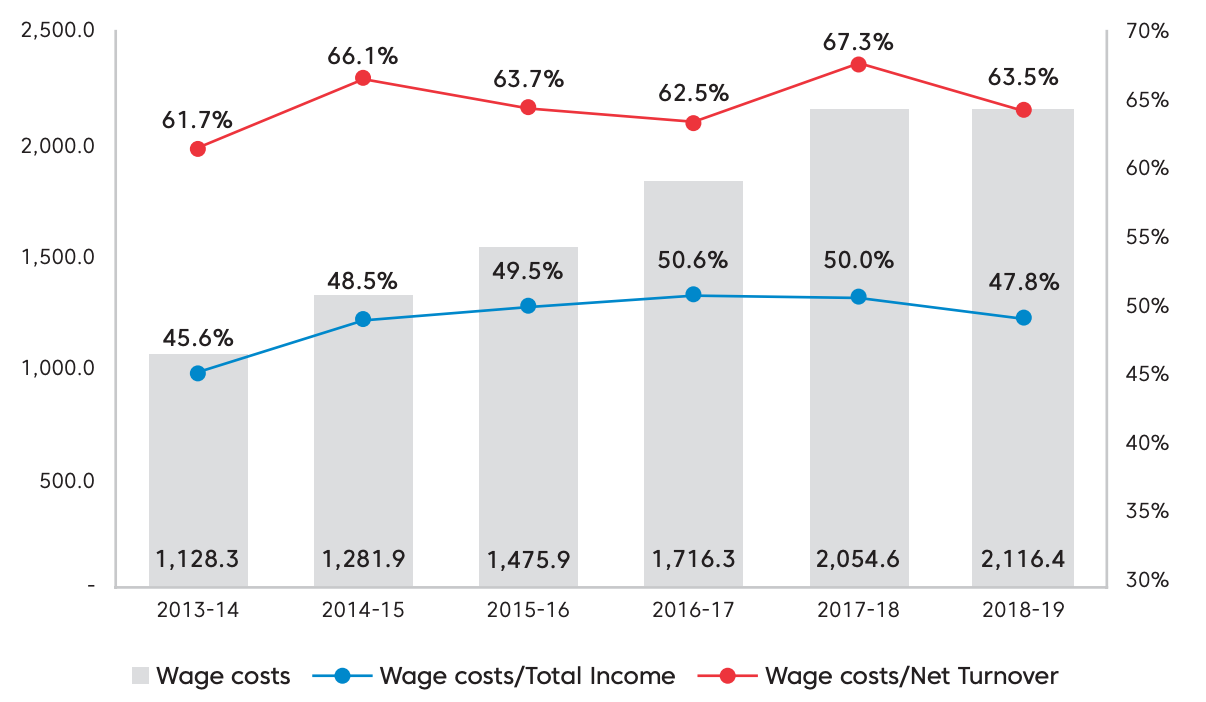
\includegraphics[scale=.5]{img/wage_spain.png}
    \caption{Stipendi La Liga}
    \label{wage_spain}
\end{figure}
La figura mostra come nonostante l'aumento del costo degli stipendi sul totale dei costi, il rapporto con il fatturato vada di anno in anno
a decrescere, mostrando ancora una volta come il campionato spagnolo sia in crescita economica. Un risultato nuovamente positivo \'e stato
sicuramente influenzato dal \emph{\textbf{Salary Cap}} introdotta nel 2013 da parte del CdS \footnote{Wikipedia: Consejo Superior de Deportes – il massimo organo sportivo a livello nazionale}.
Questa nuova riforma ha il campito di porre dei limiti alle spese dei club riguardo gli stipendi e in generale tutti i costi connessi ai calciatori,
questo per evitare problematiche presenti ad esempio in Francia dove club con forti disponibilit\'a economiche gareggiano incontrastati nel Paese.\\
Dovendo fornire un commento/conclusione all'analisi appena svolta \'e possibile affermare come La Liga sia innegabilmente in crescita da 6 
anni a questa parte, essendo il secondo campionato pi\'u visto al mondo con 2663 mln di spettatori, dietro solo la Premier League a quota 
3200 mln \footnote{Premier League: https://www.premierleague.com/news/1280062}, tuttavia bisogna comunque prestare attenzione alle attivit\'a
delle squadre pi\'u importanti come per esempio il Barcellona, che in pochi anni a partire dal 2018 si ritrover\'a in una situazione di
elevato debito e costretta quindi a prendere decisioni molto forti (addio di Lionel Messi, storico calciatore del Club, vincitore di 7 Palloni d'Oro,
il pi\'u grande riconoscimento personale Europeo).\newline
Come ultimo elemento compreso in questa prima analisi suddivisa per Paesi troviamo l'\textbf{Inghilterra}. In questo Paese il calcio 
\'e una vera e propria colonna portante, capace di generare ricavi per 5440mln€\footnote{https://www2.deloitte.com/global/en/pages/about-deloitte/articles/annual-review-of-football-finance.html}
nella stagione 2017/2018. Il punto di forza \'e sicuramente legato alla vastissima diffusione dei diritti tv che compongono il fattore ricavi
del 59\% ma \'e anche, sopratutto, una questione di lingua dato che l'inglese \'e la lingua pi\'u diffusa in tutto il mondo.\newline
Iniziando a presentare i dati riguardanti l'analisi, la societ\'a Deloitte tramite l'\emph{Annual Review of Football Finance} mostra
l'andamento dei 5 maggiori campionati europei e si sofferma inoltre su quello inglese. Questo report mostra come in solo 3 anni i \textbf{ricavi} 
dei club di \emph{Premier League}, il primo campionato inglese, siano aumentati del 41.71\% passando da 3639mln£ a 5157mln£ valori a cui solo
la Bundesliga riesce quantomeno ad avvicinarcisi. Il punto di forza, come gi\'a affermato prima, \'e sicuramente i ricavi generati dai diritti
tv che compongono ogni anni pi\'u della met\'a dei ricavi totali; anche la parte denominata \emph{Commercial} non \'e da meno, con valori
che si aggirano sempre intorno ai 1500mln£. Il vero problema per\'o si presenta se si va a confrontare i ricavi dei cosiddetti \emph{Big Six}, 
i 6 club che hanno fatto la storia del campionato: Arsenal, Manchester City, Manchester United, Tottenham, Chelsea e Liverpool con i ricavi
generati dalle altre societ\'a.
\begin{figure}
    \centering
    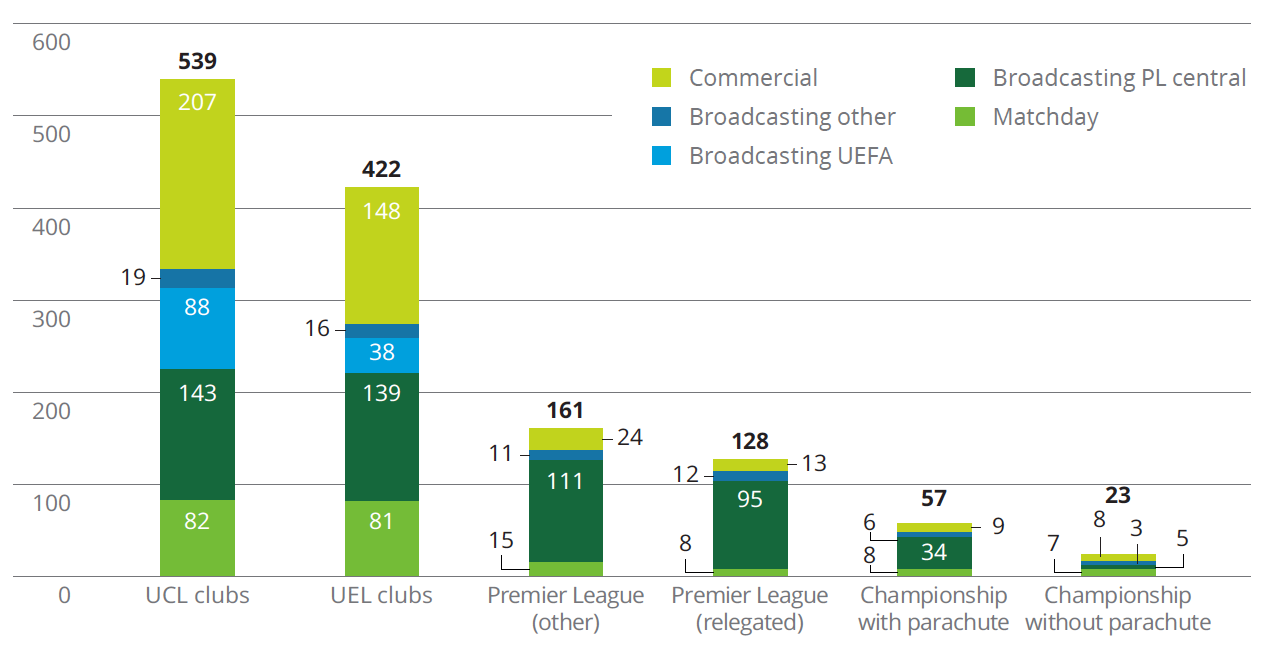
\includegraphics[scale=0.5]{img/ricavi_premier.png}
    \caption{Confronto ricavi dei club di Premier League divisi per gruppi}
    \label{ricavi_premier}
\end{figure} 
La figuta \ref{ricavi_premier} permette di visualizzare immediatamente questa differenza. L'ultima classificata tra i \emph{Big Six},
l'Arsenal ha generato ricavi 393mln£ mentre il West Ham, classificatosi settimo e quindi una posizione immediatamente sotto l'Arsenal, ha 
prodotto per 193mln£, una differenza di ricavi di 200mln£ con una sola posizione in classifica di distacco. Nel grafico sono inoltre riportati
i club retrocessi "con paracadute", un sistema che tramite i diritti di trasmissione aiuta economicamente i club nelle posizioni
pi\'u basse della classifica.\newline
Sempre all'intrerno dell'analisi fatta da Deloitte \'e contenuto un approfondimento sugli \textbf{stipendi}. Anche in questo caso, se a
primo impatto i dati non sembrano preoccupare, se si analizzano a fondo si pu\'o notare come gi\'a dalla stagione 2018/2019 ci fossero segni
di preoccupazione. Il peso degli stipendi per i club della Premier League in quella stagione ammontava a 3155mln£, il 61\% dei ricavi contro il 
59\% dell'anno precedente. Questo aumento ha fatto si che si presentassero alla fine dell'esercizio ben 6 club con una perdita operativa, il 
peggior risultato dal 2012/2013.\newline
Da questa prima analisi generale \'e emerso come, in tutti i Paesi, il sistema calcio prima del COVID19 fosse in grande espansione ma 
questa espansione era causata da grandi somme di denaro investite senza una reale certezza che si sarebbe andato a creare un ritorno economico,
Questa pratica, aggravata dall'avvento della pandemia, \'e sfociata in quello che oggi \'e diventato \textbf{un settore non pi\'u sostenibile}.
\section{Analisi per Club}
\subsection{Juventus}
\end{interlinea}
\end{document}

